\documentclass{standalone}
\usepackage{tikz}
\usepackage{ctex,siunitx}
\setCJKmainfont{Noto Serif CJK SC}
\usepackage{tkz-euclide}
\usepackage{amsmath}
\usetikzlibrary{patterns, calc,3d}
\usetikzlibrary {decorations.pathmorphing,decorations.pathreplacing,decorations.shapes,}
\tikzset{label style/.append style={font=\small}}
\begin{document}
\small
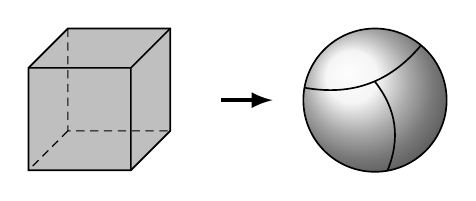
\begin{tikzpicture}[>=latex,scale=1.3]
  \begin{scope}
    \draw[semithick,fill=lightgray](1,0,0)--(1,1,0)--(0,1,0)--(0,1,1)--(0,0,1)--(1,0,1)--cycle;
    \draw[semithick](0,1,1)--(1,1,1)--(1,1,0)(1,1,1)--(1,0,1);
    \draw[densely dashed](0,1,0)--(0,0,0)--(1,0,0)(0,0,0)--(0,0,1);
  \end{scope}
  \draw[ultra thick,->](1.5,0.3)--++(0.5,0);
  \begin{scope}[xshift=3cm,yshift=3mm]
    \draw[semithick,ball color=lightgray!20](0,0)circle(0.7);
    \draw[semithick](170:0.7)to[bend right](50:0.7)(90:0.18)to[bend left](280:0.7);
  \end{scope}
\end{tikzpicture}
\end{document}